% Common notations, theorems and procedures

\section{Notations\label{section:notations}}


The following notations will be used throughout this document:
\begin{itemize}

\item  $+$, $-$ and  $\times$ denote the usual
mathematical operations.

\item $\oplus$, $\ominus$ and $\otimes$ denote the
corresponding floating-point operations in IEEE-754 double precision,
in the IEEE-754 \emph{round to nearest} mode.

\item $\epsilon$ (usually with some index) denotes an error and
  $\delta$ (with the same index) denotes a bound on this error.

\item $\epsilon_{-k}$ -- with a negative index -- denotes an error bounded by $2^{-k}$.
  
\item For a floating-point number $x$, the value of the least
  significant bit of its mantissa is classically denoted $\ulp(x)$.

\end{itemize}




\section{Common C procedures  for double-precision numbers\label{section:commonCdouble}}

\subsection{Sterbenz Lemma}

\begin{theorem}[Sterbenz Lemma~\cite{Ste74,Gol91}]
\label{sterbenz}
If $x$ and $y$ are floating-point numbers, and if ${y}/{2} \leq x \leq 2y$ then $x\ominus y$ is computed exactly, without any rounding error.
\end{theorem}


\subsection{Double-precision numbers in memory\label{section:memory}}

A double precision floating-point number uses $64$ bits. The unit of memory in most current
architectures is a 32-bit word. The
order in which the two $32$ bits words of a double are stored in memory  depends on
the architecture. An architecture is said \emph{Little Endian} if the
lower part of the number is stored in memory at the smallest address;
It is the case of the x86 processors. Conversely, an architecture
with the high part of the number stored in memory at the smallest
address is said \emph{Big Endian}; It is the case of the PowerPC
processors.


The following code extracts the upper and lower part from a double
precision number $x$.

\begin{lstlisting}[label={chap0:lst:endian},
  caption={Extract upper and lower part of a double precision number $x$},firstnumber=1]
/* LITTLE_ENDIAN/BIG_ENDIAN are defined by the user or  */
/* automatically by tools such as autoconf/automake.   */

#ifdef LITTLE_ENDIAN
#define HI(x) *(1+(int*)&x)
#define LO(x) *(int*)&x
#elif BIG_ENDIAN
#define HI(x) *(int*)&x
#define LO(x) *(1+(int*)&x)
#endif
\end{lstlisting}



\subsection{Conversion from floating-point to integer}

\begin{theorem}[Conversion floating-point to integer]
  The following algorithm, taken from \cite{AMDoptim2001}, converts a
  double-precision floating-point number $d$ into a 32-bit
  integer $i$ with rounding to nearest mode.
\begin{lstlisting}[label={chap0:lst:conversion2},caption={Conversion from FP to int},firstnumber=1]
#define DOUBLE2INT(i, d) \
  {double t=(d+6755399441055744.0); i=LO(t);}
\end{lstlisting}
\end{theorem}
This algorithm adds the constant $2^{52}+2^{51}$ to the floating-point
number to put the integer part of $x$, in the lower part of the
floating-point number.  We use $2^{52}+2^{51}$ and not $2^{52}$,
because the value $2^{51}$ is used to contain possible carry
propagations with negative numbers.









\section{Common C procedures for double-double arithmetic\label{section:commonCdoubledouble}}

In this section, we give the basic algorithms for computing with
numbers represented the sum of two floating-point numbers (or
\emph{double-double} numbers). 

The algorithms are given as plain C functions, but it may be
preferable, for performance issue, to implement them as macros, as in
\texttt{libnultim}.  Sometimes, the code offers both versions,
selected by the \texttt{DEKKER\_AS\_FUNCTIONS} constant which is set
by default to 1 (functions).


\subsection{Exact sum algorithm {Add12}}

This algorithm is also known as the Fast2Sum algorithm in the litterature.
\begin{theorem}[Exact sum~\cite{Knu73, Boldo2001}]
  Let $a$ and $b$ be floating-point numbers, then the following method
  computes two floating-point numbers $s$ and $r$, such that $s+r =
  a+b$ exactly, and $s$ is the floating-point number which is closest
  to $a+b$.

\begin{lstlisting}[label={lst:Add12Cond},caption={Add12Cond},firstnumber=1]
void Add12Cond(double *s, double *r, a, b) 
{
  double z;
  s = a + b;            
  if ((HI(a)&0x7FF00000)> (HI(b)&0x7FF00000)){  
    z = s - a;           
    r = b - z;           
  }else {                 
    z = s - b;           
    r = a - z;           
  } 
}                         
\end{lstlisting}
This algorithm requires $3$ floating-point additions, $2$ masks and $1$ test over integer.
\end{theorem}


If we are able to prove that  the exponent of $a$ is always greater than that
of $b$, then the previous algorithm to perform an exact addition of 2
floating-point numbers becomes :
\begin{lstlisting}[label={lst:Add12},caption={Add12},firstnumber=1]
void Add12Cond(double *s, double *r, a, b) 
{
  double z;
  s = a + b;            
  z = s - a;  
  r = b - z; 
}            
\end{lstlisting}
The cost of this algorithm is $3$ floating-point additions.






\subsection{Exact product algorithm {Mul12}}

This algorithm is sometimes  also known as the Dekker algorithm \cite{Dek71,Knu73}.

\begin{theorem}[Restricted exact product]
  Let $a$ and $b$ be two double-precision floating-point numbers, with
  53 bits of mantissa. Let $c=2^{\frac{\lceil 53 \rceil}{2}}+1$.
  Assuming that $a<2^{970}$ and $b<2^{970}$, the following procedure
  computes the two floating-point numbers $rh$ and $rl$ such that $rh
  + rl = a + b$ with $rh = a \otimes b$:
\begin{lstlisting}[label={lst:Mul12},caption={Mul12},firstnumber=1]
void  Mul12(double *rh, double *rl, double u, double v){
  const double c = 134217729.;   /*  1+2^27 */ 
  double up, u1, u2, vp, v1, v2;

  up = u*c;        vp = v*c;
  u1 = (u-up)+up;  v1 = (v-vp)+vp;
  u2 = u-u1;       v2 = v-v1;
  
  *rh = u*v;
  *rl = (((u1*v1-*rh)+(u1*v2))+(u2*v1))+(u2*v2);
}
\end{lstlisting}
\end{theorem}

The cost of this algorithm is $10$ floating-point
additions and $7$ floating-point multiplications.



The condition $a<2^{970}$ and $b<2^{970}$ prevents overflows when
multiplying by $c$. If it cannot be proved statically, then we have to
first test $a$ and $b$, and prescale them so that the condition is
true.


\begin{theorem}[Exact product]
  Let $a$ and $b$ be two double-precision floating-point numbers, with
  53 bits of mantissa. Let $c=2^{\frac{\lceil 53 \rceil}{2}}+1$.
  Assuming that $a<2^{970}$ and $b<2^{970}$, the following procedure
  computes the two floating-point numbers $rh$ and $rl$ such that $rh
  + rl = a + b$ with $rh = a \otimes b$:

\begin{lstlisting}[label={lst:Mul12Cond},caption={Mul12Cond},firstnumber=1]
void Mul12Cond(double *rh, double *rl, double a, double b){
  const double two_970 = 0.997920154767359905828186356518419283e292;
  const double two_em53 = 0.11102230246251565404236316680908203125e-15;
  const double two_e53  = 9007199254740992.;
  double u, v;

  if (a>two_970)  u = a*two_em53; 
  else            u = a;
  if (b>two_970)  v = b*two_em53; 
  else            v = b;

  Mul12(rh, rl, u, v);

  if (a>two_970) {*rh *= two_e53; *rl *= two_e53;} 
  if (b>two_970) {*rh *= two_e53; *rl *= two_e53;} 
}\end{lstlisting}
\end{theorem}

The cost in the worst case is then $4$ tests over integers,
$10$ floating-point additions and $13$ floating-point multiplications.


Finally, note that a fused multiply-and-add provides the Mul12 and
Mul12Cond in only two instructions \cite{CorneaHarrisonTang2002}. Here
is the example code for the Itanium processor.

\begin{lstlisting}[label={lst:Mul12CondFMA},caption={Mul12 on the Itanium},firstnumber=1]
#define Mul12Cond(rh,rl,u,v)                          \
{                                                     \
  *rh = u*v;                                          \
  /* The following means: *rl = FMS(u*v-*rh) */       \
  __asm__ __volatile__("fms %0 = %1, %2, %3\n ;;\n"   \
                       : "=f"(*rl)                    \
                       : "f"(u), "f"(v), "f"(*rh)     \
                       );                             \
}
#define Mul12 Mul12Cond
\end{lstlisting}



\subsection{Double-double addition {Add22}}
  
This algorithm, also due to Dekker \cite{Dek71}, computes the sum of
two double-double numbers as a double-double, with a relative error
smaller than $2^{-103}$.

\begin{lstlisting}[label={Add22},caption={Add22},firstnumber=1]
void Add22(double *zh, double *zl, double xh, double xl, double yh, double yl)
{
double r,s;

r = xh+yh;
s = (ABS(xh) > ABS(yh))? (xh-r+yh+yl+xl) : (yh-r+xh+xl+yl);
*zh = r+s;
*zl = r - (*zh) + s;
}
\end{lstlisting}

Here ABS is a macro that returns the absolute value of a floating-point number.




\subsection{Double-double multiplication {Mul22}}
  
This algorithm, also due to Dekker \cite{Dek71}, computes the product of
two double-double numbers as a double-double, with a relative error
smaller than $2^{-102}$.

\begin{lstlisting}[label={Mul22},caption={Mul22},firstnumber=1]
void Mul22(double *zh, double *zl, double xh, double xl, double yh, double yl)
{
double mh, ml;

  const double c        = 134217729.;                /* 0x41A00000, 0x02000000 */ 
  double up, u1, u2, vp, v1, v2;

  up = xh*c;        vp = yh*c;
  u1 = (xh-up)+up;  v1 = (yh-vp)+vp;
  u2 = xh-u1;       v2 = yh-v1;
  
  mh = xh*yh;
  ml = (((u1*v1-mh)+(u1*v2))+(u2*v1))+(u2*v2);

  ml += xh*yl + xl*yh;
  *zh = mh+ml;
  *zl = mh - (*zh) + ml;
}  
\end{lstlisting}

Note that the bulk of this algorithm is a \texttt{Mul12(mh,ml,xh,yh)}.

Note that our algorithms will sometimes need to multiply a double by a
double-double. In this case we use \texttt{Mul22} with one of the
arguments set to zero, which only performs one useless multiplication
by zero and one useless addition.




\section{Test if rounding is possible\label{section:testrounding}}

We assume here that an evaluation of $y=f(x)$ has been computed with a
total relative error smaller than $\delta$, and that the result is
available as the sum of two non-overlapping floating-point numbers
$y_h$ and $y_l$ (as is the case if computed by the previous
algorithms). This section gives and proves algorithms for testing if
$y_h$ is the correctly rounded value of $y$.




\subsection{Rounding to the nearest}

\begin{theorem}[Correct rounding of a double-double to the nearest double, avoiding denormals]
\label{th:roundingRN1}
~\\
      Let $y$ and $\delta$ be real numbers, and $e$, $y_h$ and $y_l$ be
  floating-point numbers such that 
  \begin{itemize}
  \item $y_h=y_h\oplus y_l$,
  \item none of $y_h$ and $y_l$ is a  NaN.
  \item $|y_h|\ge 2^{-1022+53}$ 
  \item $|y_h+y_l - y| < \delta.|y|$
  \item $0< \delta \le 2^{-53-k}$ with $k\ge 2$ integer
  \item $e\ge 1+  \dfrac{2^{53+k+1}\delta}{(2^{k}-1)(1-2^{-53})}$
\end{itemize}

The following test determines whether $y_h$ is the
  correctly rounded value of $y$ in  round to nearest mode.

\begin{lstlisting}[
  firstnumber=1]
if( (*@$y_h$@*) == ((*@$y_h$@*) + ((*@$y_l$@*)*e)) )
  return (*@$y_h$@*);
else /* more accuracy is needed, lauch accurate phase */
\end{lstlisting}
\end{theorem}

\begin{proof}
  The theorem holds if $y_h$ is $\pm \infty$.
  
  It also holds if $y_h$ is a denormal: in this case $y_l$ is zero, so
  the correctly rounded result is $y_h$, and the test is true. In the
  following we therefore assume that $y_h$ is a normal number. We also
  assume that $y\ge0$ (so $y_h\ge0$), as the other case is symmetric.
  
  Let us note $u=\ulp(y_h)$. By definition of the \ulp, we have $y_h
  \in [2^{52}u, (2^{53}-1)u]$, which implies $y<2^{53}u$ as $y < y_h + y_l + \delta y
  < (2^{53}-1)u +\frac{1}{2}u +\frac{1}{2}u$.

  What we want to prove is that if the test is true, then $y_h =
  \round(y)$. We will prove that  if the test is true, then $|y_l-\frac{1}{2}u| > 2^{53}\delta
  u$, which implies $|y_l-\frac{1}{2}u| > \delta y$, which implies
  that we are not in a difficult case for correct rounding to the
  nearest, so $y_h = \round(y)$.

  Consider the case when $y_l$ is positive:  $0\le y_l \le \frac{1}{2}u$.

  If $0 \le y_l < (\frac{1}{2} - \frac{1}{2^{k+1}})u$, then since
    $|\delta|<2^{-53+k}$ we are in an easy case for rounding to the
    nearest, and $y_h = \round(y)$ regardless of the result of the test.

    Now consider the case when $y_l \ge (\frac{1}{2} - \frac{1}{2^{k+1}})u$.
   % = \frac{2^{k}-1}{2^{k+1}}u
    Remark that the condition $|y_h|\ge 2^{-1022+54}$ ensures that
    $\frac{1}{2}u$ is a normal number, so in this case
    $y_l$ is a normal number. As $e>1$ this ensures that
    $$y_l\times e(1-2^{-53})\ \le\ y_l \otimes e\ \le\ y_l\times e(1+2^{-53})$$


  Suppose that the test is true ($y_h \oplus y_l \otimes e = y_h$). 
  With IEEE-54 compliant rounding to
  nearest, this implies $|y_l \otimes e|
  \le \frac{1}{2}u$, which in turn implies $|y_l \times e|
  (1-2^{-53}) \le \frac{1}{2}u$, as $y_l$ is a normal number and $e>1$. 
  
  We get $y_l \times (1+e-1)(1-2^{-53}) \le \frac{1}{2}u$, or
  \begin{equation}
  \frac{1}{2}u - y_l \ge y_l (e-1)(1-2^{-53})\label{eq:prooftestRN2}
  \end{equation}  

(\ref{eq:prooftestRN2}) implies
    $\frac{1}{2}u - y_l \ge \frac{2^{k}-1}{2^{k+1}} (e-1)(1-2^{-53}) >
    2^{53}\delta u$, from $e\ge 1+
    \frac{2^{53+k+1}\delta}{(2^{k}-1)(1-2^{-53})}$.

  The case when $y_l$ is negative is similar.
\end{proof}



\begin{theorem}[Correct rounding of a double-double to the nearest double, general case]
\label{th:roundingRN2}
~\\
  Let $y$ and $\delta$ be real numbers, and $e$, $y_h$ and $y_l$ be
  floating-point numbers such that 
  \begin{itemize}
  \item $y_h=y_h\oplus y_l$,
  \item none of $y_h$ and $y_l$ is a  NaN.
  \item $|y_h+y_l - y| < \delta.|y|$
  \item $0< \delta \le 2^{-53-k}$ with $k\ge 2$ integer
  \item $e\ge 1+  \dfrac{2^{53+k+2}\delta}{2^{k}-1}$
\end{itemize}

The following test determines whether $y_h$ is the
  correctly rounded value of $y$ in  round to nearest mode.

\begin{lstlisting}[firstnumber=1]
if( (*@$y_h$@*) == ((*@$y_h$@*) + ((*@$y_l$@*)*e)) )
  return (*@$y_h$@*);
else /* more accuracy is needed, lauch accurate phase */
\end{lstlisting}
\end{theorem}

\begin{proof}
  The proof is identical to the previous theorem, with the exception
  that we cannot ensure anymore that $y_l$ will not be a denormal.
  Therefore the relative error on $y_l\times e$ may be as high as
  $\frac{1}{2}$, and the condition on $e$ is reinforced accordingly.
\end{proof}


\subsubsection*{Notes}

\begin{itemize}
\item In general we will target values of $\delta$ in the order of
  $2^{-53-10}$ to balance the execution times of the quick and
  accurate phases. In this case, using the first theorem almost divides
  by two the frequency of calls to the accurate phase. 
\item It is not obvious that a fused multiply-and-add may be used for
  the computation of $y_h+y_l\times e$, but the proof should be easy
  to adapt to this (more accurate) operation.
\end{itemize}



\subsection{Rounding up}

\begin{theorem}[Correct rounding of a double-double to a double]
  Let $y$ and $\delta$ be real numbers, and $e$, $y_h$ and $y_l$ be
  floating-point numbers such that 
  \begin{itemize}
  \item $y_h=y_h\oplus y_l$,
  \item none of $y_h$ and $y_l$ is a  NaN.
  \item $|y_h+y_l - y| < \delta.|y|$
  \item $0< \delta \le 2^{-53-k}$ with $k\ge 2$ integer
  \item $e\ge 1+  \dfrac{2^{53+k+1}\delta}{(2^{k}-1)(1-2^{-53})}$
\end{itemize}

The following test determines whether $y_h$ is the
  correctly rounded value of $y$ in  round to nearest mode.

\begin{lstlisting}[label={roundingtonearest},
  caption={Test for correct rounding to nearest},
  firstnumber=1]
if( (*@$y_h$@*) == ((*@$y_h$@*) + ((*@$y_l$@*)*e)) )
  return (*@$y_h$@*);
else /* more accuracy is needed, lauch accurate phase */
\end{lstlisting}
\end{theorem}

\subsection{Rounding down}

TODO







\section{The Software Carry Save library}

The software carry-save internal representation of multiple-precision
numbers was designed specifically for simple and fast implementations
of addition and multiplication in the 100-500 bit precision range, as
required by the \accurate\ phase of our algorithms. More details on
software carry-save are available in \cite{DefDin2002,DinDef2003}.

The parameters of \scslib\ are set up so that all the operators offer
a relative error better than $2^{-208}$.  This is a large overkill for
all the functions in \crlibm, as the worst cases computed by Lefevre
never require more than 158 bits of accuracy. This enables simple
proofs for the second steps, assuming the operators in \scslib\ are
correct.

Another feature that makes accuracy proofs simple when using \scslib\ 
is the following: The range of SCS numbers includes the range of IEEE
double-precision numbers, including denormals and exceptional cases.
Conversions between SCS format and IEEE-754 doubles, as well as
arithmetic operations, follow the IEEE rules concerning the
exceptional cases. SCS doesn't ensure correct rounding, but provides
conversions to doubles in the four IEEE-754 rounding modes, wich is
enough for the purpose of \crlibm.

However, a formal proof of correctness of the \scslib\ operators
remains to be done. Currently there is nothing more than good
confidence based on the simplicity of the code.


\subsection{The SCS format}

 A MP number is represented in the proposed format as a
\emph{Software Carry Save} (SCS) structure $R$, depicted on
Figure~\ref{fig:scsrepresentation} and composed of the following
fields:
\begin{description}
\item[\emph{R.digits[$n_r$]}] A table of $n_r$ digits with $m_r$ bits
  of precision. These digits can in principle be either integer or FP
  machine numbers, however integer is always faster and simpler. We
  will not mention FP digits anymore here, the interested reader is
  referred to \cite{DefDin2002,DinDef2003}.
\item[\emph{R.index}] An integer storing the index of the first digit
  in the range of representable numbers, as depicted on
  Figure~\ref{fig:representation};
 \item[\emph{R.sign}] A sign information.  
\end{description}

\begin{figure}[h]
\begin{center}
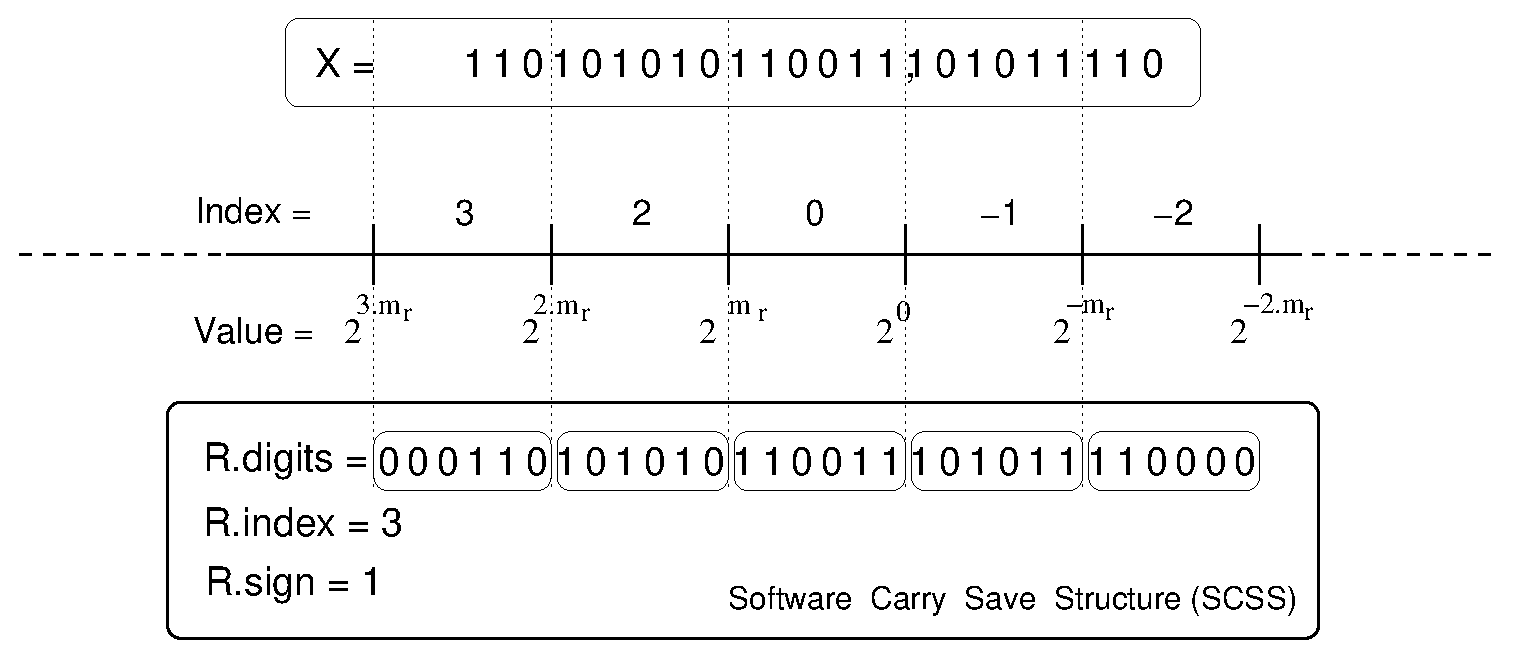
\includegraphics[width=0.7\textwidth]{fig_scs/exponent_representation} % image file name
\caption{The proposed format \label{fig:scsrepresentation}}
\end{center}
\end{figure}
  
In other words, the value  $x$ of a representation $R$  is:
\begin{equation}
\label{eqn4}
x = R.sign \times \sum_{j=1}^{n_r} R.digits[j] \times 2^{m_r * (R.index - j)}
\end{equation}

In such a \emph{normal} SCS number $R$, the bits from $m_I$ to $m_r$
of the $R.digits$ fields are thus set to zero. They will be exploited
by the algorithms to store temporary \emph{carry} information, and are
therefore called \emph{carry-save} bits. An SCS number where these
bits are non-zero is said to be non-normal.

The values of the parameters for use in \crlibm\ is $n_r=8$ digits of
$m_i=30$ bits stored on $m_r=32$-bit words. The worst-case precision
that this format may hold is when the most significant digit is equal
to $1$, meaning that an SCS numbers holds only $1+7\times 30=211$
significant digits.


\subsection{Arithmetic operations\label{sec:ops}}


\subsubsection{Conversion from double to SCS}
 A first method for converting a double precision floating
point number $d$ into an SCS representation is to extract the
exponent $d_{exp}$ from $d$, and then determine the corresponding
$R.index$ as the integer part of
$\frac{d_{exp}}{2^{m_r}}$.

Another method uses a variable number of multiplications by
$2^{m_r}$ or $2^{-m_r}$. This method is faster than the previous one
when the exponent of $d$ is close to $0$.

After testing both methods in \crlibm, the first method was preferred.


\subsubsection{Addition and subtraction}

The addition of two SCS numbers of the same sign consists in aligning,
then adding digits of the same order. Thanks to the carry-save bits,
all these additions will be \emph{exact} and \emph{independent}.
However the result will usually not be a normal SCS number: the sums
will have overflown in the carry-save bits. A \emph{renormalization}
procedure is presented in section \ref{renorm} to propagate these
carry bits and get again a normal SCS number.  However, the advantage
of SCS representation is that many SCS numbers can be summed before
needing to perform this expensive step (up to 7 with the choice of
parameters made in \crlibm).

The subtraction (addition of two numbers of opposite signs) is very
similar to the addition algorithm. It may also classically lead to a
cancellation, which may need an update of the index of the result.
However, as in other floating-point formats, a subtraction involving a
a cancellation is exact.

Although all the digit operations are exact, the addition or
subtraction of two numbers also classically involves a rounding error,
due to aligning the digits of same magnitude. For performance reason
this rounding is a truncation, so the worst-case relative error is one
ulp of the least accurate representable number, or $2^{-211}$.




%---------------- 
% MULTIPLICATION
%----------------
\subsubsection{Multiplication}

The multiplication of two normal SCS numbers involves the operations
depicted on the Figure \ref{fig:scsmultiplication}: The partial
products are computed (in parallel) and summed in columns. The
parameters are set up so that none of these operation overflow. Again,
the result is not a normal SCS number, and a renormalization procedure
(described below) has to be applied to empty the carry bits. However,
a few additions may follow a multiplication before this
renormalization, which allows for further optimization of algorithms
using SCS arithmetic. For instance, a polynomial evaluation can be
implemented with a renormalization after one multiplication and one
addition.

\begin{figure}[h]
\begin{center}
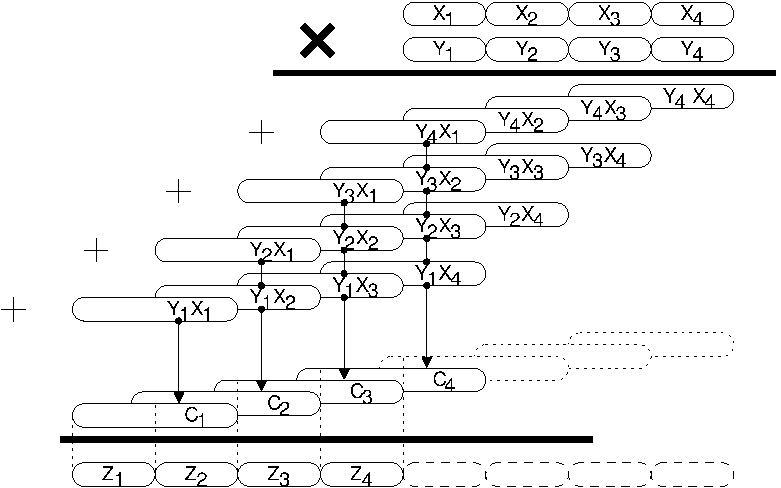
\includegraphics[width=0.7\textwidth]{fig_scs/multiplication}
\caption{SCS multiplication \label{fig:scsmultiplication}}
\end{center}
\end{figure}

Here also, a rounding error is involved when two $n_r$-digit numbers
are multiplied if the result is to fit on $n_r$ digits. The actual
implementation tests if the most significant digit ($z_1$ on
Figure~\ref{fig:multiplication}) is null, in which case the index of
the result is that of $z_2$.

If the whole of the computations of
Figure~\ref{fig:scsmultiplication} are implemented, the worst case
for relative accuracy is again $2^{-211}$. However a further
optimization is to avoid computing the columns of lower magnitude, at
the expense of an increase in the rounding error. More specifically,
we compute 9 columns instead of 16.  The wors case is now when $z_1$
is null, in which case the relative error correspond to the truncation
of the 8 leftmost columns, whose maximum value is smaller than 3 ulps
of the SCS result. Therefore the relative error of the multiplication
is bounded by $2^{-208}$ with this optimization, which is still a
large overkill for the purpose of \crlibm.

This optimization is therefore implemented if the loop are hand-unrolled.
If they are not, the increased control complexity actually degrades
performance.


\subsubsection{Renormalization (carry propagation) \label{renorm}}

Renormalization is a carry propagation from the low order to high
order digits: Starting with an initially null carry, at each step, the
previous carry is added to the current digit, and this sum is then
split into two parts using masks. The low $m_r$ bits are a digit of
the normalized result, and the upper part is the next carry.

The actual algorithm is a little bit more complex. The initial
non-normal number may not be representable exactly as a normal SCS
number, therefore the index of the normalized result may have to be
increased by one or two.  Normalization thus again involves a rounding
error. Note that this error was already taken into account in the previous
discussions of addition and multiplication.




%-----------------
% CONVERSION BACK
%-----------------
\subsubsection{Conversion from SCS to floating-point}

A few (4 in the worst case) multiplications and additions suffice to
get the FP number closest to a SCS number.  For instance, for $m_I=53$
and $m_r=26$, we need to compute $d = A.sign \times 2^{A.index \times
  m_r} \times ( A.digits[0]+ 2^{-m_r} \times A.digits[1]+ 2^{-2.m_r}
\times A.digits[2]+ 2^{-3.m_r} \times A.digits[3])$. The number
$2^{A.index \times m_r}$ is build using integer masks. The actual
implementation of this formula is slightly less simple, but this
conversion is still very fast.


\subsubsection{Mixed 32- and 64-bit arithmetics}

An improvement implemented in \scslib\ was the combined use of integer 32- and 64-bit
arithmetics as follows: 

\begin{itemize}
\item MP digits are stored as 32-bit numbers where only a few bits are
  reserved for carries. This removes the main problem of the initial
implementation \cite{Dinechin2002b}, namely its memory inefficiency.

\item Addition uses 32-bit arithmetic. 

\item In the MP multiplication, the partial products are products of
  two 32-bit digits, which are 64-bit numbers. The column sums need
  thus to be computed using 64-bit arithmetic. This can be expressed
  in the C language in a non-ANSI-C99, but de-facto standard way, as
  follows: 32-bit numbers have the \texttt{unsigned int} type; 64-bit
  numbers have the \texttt{unsigned long long int} type. When
  multiplying two digits, one is first cast into this 64-bit type.
  
  For UltraSPARC architectures (detected at build time) the
  conversion is to floating-point, but we will not detail this
  peculiarity further.
\end{itemize}


This works well because all modern processors either have 64-bit
integer units, or offer instructions which store the 64-bit product of
two 32-bit integers into two 32-bit registers. The compiler does the
rest well, because it is conceptually simple: casting unsigned 32-bit
into unsigned 64-bit is trivial; 64-bit addition is translated
straightforwardly into one 32-bit \emph{add} followed by one 32-bit
\emph{add-with carry}.




\subsubsection{Implementation considerations}

For portability purposes, the implemention uses ANSI C as defined by
the C99 standard, and tries to use a recent version of \texttt{gcc}.
We could not exhibit a case where a native compiler from the processor
vendor (Intel or Sun) gave significantly better results than
\texttt{gcc}, which is probably a consequence of the simplicity of our
code.

However, when tuning for performance, we observed that the same code
which was efficient on one processor could lead to very poor results
on another.  Usually, this difference can be traced down to the
capabilities of the processor itself. The typical example is the
knowingly poor integer multiplication on UltraSPARC II. Sometimes
however, the processor should be able to perform well, and it is the
processor-specific backend of the compiler which is to blame, which
can be checked by observing the assembly code produced.  A typical
example is the casting of 32-bits digits to 64-bit arithmetic (or to
an FP number in the case of the UltraSPARC) in the multiplication
algorithm. In these cases we tried to change the programming style in
a way that works well on all processors. Sometimes it wasn't possible,
in which case the code contains, along with a generic version, several
processor-specific tricky versions of the problematic operation,
selected at compile time thanks to the GNU \texttt{automake/autoconf}
tools.


More surprisingly, we were disappointed by the higher-level
capabilities of the compilers, especially at unrolling loops. Our code
exhibits many small \texttt{for} loops whose size is known at
compile-time (usually $n$). This is the ideal situation for loop
unrolling, a technique well known and described in most textbooks on
compiler design. Options exist in most compilers to turn on this
optimisation. Unfortunately, leaving loop unrolling to the compiler
gives very poor results, even when compared to the non-unrolled case.
Since unrolling the loops by hand in the C code takes a few minutes,
we did it for the version of the library which we use ($m=30$, $n=8$).
It marginally increases the code sizes for this small $n$, and
sometimes provides a twofold improvement on speed, depending of the
processor. Of course, this is not satisfactory: We don't want to do it
for all values of $n$, nor do we want to study for each processor the
tradeoffs involved as $n$ increase. We expect however future compilers
to handle unrolling better, and we were surprised that no compiler had
a clear edge on the other in this respect. Some argue, however, that
this issue is pointless, as superscalarity, along with register
renaming and branch prediction inside modern processors, sum up to the
equivalent of dynamic unrolling of the code. In our tests (in 2003), it
doessn't: unrolling does bring a speed-up.








\section{Common Maple procedures \label{section:commonMaple}}


\subsection{Conversions}

Procedure \texttt{nearest} provides the closest IEEE-double number
from input value \texttt{u}.

\begin{lstlisting}[caption={nearest},firstnumber=1]

nearest := proc(u)
local arrondi, signe, x, exposant, mantisseinfinie, mantisse;
Digits:=200:
if u = 0 then arrondi := 0
else 
  if (u < 0) then signe := -1; x := -u else signe := 1; x := u fi;
  exposant := floor(evalf(log(x)/log(2.0)));
  mantisseinfinie := x*2^(52-exposant);
  if frac(mantisseinfinie) < 0.5 then mantisse := round(mantisseinfinie)
   else
     mantisse := floor(mantisseinfinie);
     if type(mantisse,odd) then mantisse := mantisse+1 fi;
   fi;
   arrondi := signe*mantisse*2^(exposant-52)
fi;
arrondi;
end:
\end{lstlisting}



Procedure \texttt{IEEEdouble} returns the exponent, the mantissa and the
binary conversion of the closest IEEE-double number of input value \texttt{x}.

\begin{lstlisting}[caption={IEEEdouble},firstnumber=1]
IEEEdouble:=proc(x) local signe, logabsx, exposant, mantisse, mantisseinfinie, resultat; 
 Digits:=200;
if (x=0) then [0,0,0]; 
else 
 if (x<0) then signe:=-1:
 else signe:=1:
 fi:
 exposant := floor(evalf(log(signe*x)/log(2.0)));
 if (exposant>1023) then mantisse:=infinity:
 elif (exposant<-1022) then mantisse:=0:
 else 
  mantisseinfinie := signe*x*2^(52-exposant);
  if frac(mantisseinfinie) <
0.5 then mantisse := round(mantisseinfinie)
   else
     mantisse := floor(mantisseinfinie);
     if type(mantisse,odd) then mantisse := mantisse+1 fi;
   fi;
 mantisse:= signe*mantisse*2**(-52);
 Digits := 53;
 resultat:=convert(mantisse*2.0^(exposant),binary);
 fi;
[exposant, mantisse, resultat];
fi;
end:
\end{lstlisting}

Procedure \texttt{hi\_lo} returns two IEEE-double numbers $x\_hi$ and $x\_lo$ so that $x = x\_hi + x\_lo + \epsilon_{-103}$.

\begin{lstlisting}[caption={hi\_lo},firstnumber=1]

hi_lo:= proc(x)
global x_hi, x_lo, res:
local tamp:
x_hi:= nearest(evalf(x)):
res:=x-x_hi:
if (res = 0) then
  x_lo:=0:
else
  x_lo:=nearest(evalf(res)):
end if;
(x_hi,x_lo);
end:
\end{lstlisting}
\vspace{0.5cm}



Procedure "ieee2Hexa" returns the closest IEEE-double number from x, in hexadecimal.

\begin{lstlisting}[caption={ieee2Hexa},firstnumber=1]

ieee2Hexa:= proc(x)
  local signe, hex1, hex2, ma, manti, expo, expos, bina, bin1, bin2, dec1, dec2;
  if(x=0) then resultat:=["00000000","00000000"];
  elif(x=-0) then resultat:=["80000000","00000000"];
  elif(x=2) then resultat:=["40000000","00000000"];
  elif(x=-2) then resultat:=["C0000000","00000000"];
  else
   ma:=IEEEdouble(x);
   expo:=ma[1]:
   if (ma[2]<0) then 
    manti:=2**64 + 2**63+(-ma[2]-1)*2**52+(expo+1023)*2**52;
   else 
     manti:=2**64 + (ma[2]-1)*2**52+(expo+1023)*2**52;
   fi:
   hex2:=convert(manti, hex); 
   hex2:=convert(hex2, string):  
  
   resultat:=[substring(hex2,2..9), substring(hex2,10..18)];
  end if;
  resultat;
end proc:
\end{lstlisting}
\vspace{0.5cm}

Procedure "Hexa2ieee" returns the decimal IEEE-double number associated with the hexadecimal enter value "hexa".

\begin{lstlisting}[caption={Hexa2ieee},firstnumber=1]

Hexa2ieee:= proc(hexa)
local dec, bin, expobin, expo, mantis, sign, hex1, hex2, hexcat;
global res;

hex1:= op(1, hexa):
hex2:= op(2, hexa):
hexcat:= cat(hex1, hex2);
dec:= convert(hexcat, decimal, hex):

if(dec >= 2**63) then
  dec = dec - 2**63:
  sign:= -1:
else
  sign:= 1:
fi;  
expo:= trunc(dec/(2**52))-1023:
mantis:= 1+frac(dec/(2**52));
res:= evalf(sign*2**(expo)*mantis);
end proc:
\end{lstlisting}


\subsection{Procedures for polynomial approximation}


Procedure \texttt{Poly\_exact2} takes in arguments a polynomial \texttt{P} and a
integer \texttt{n}. It returns a truncated polynomial, of wich coefficients
are exactly IEEE-double numbers. The \texttt{n} first coefficients are written
over 2 IEEE-double numbers.
 

\begin{lstlisting}[caption={poly\_exact2},firstnumber=1]

poly_exact2:=proc(P,n)
local i, coef, coef_t:
global deg, Q, psup, pinf, pfull:
psup:=0: pinf:=0:
Q:=[];
convert(psup, polynom): convert(pinf, polynom):
deg:=degree(P,x):
  for i from 0 to deg do
    coef:=coeff(P,x,i):
    if (coef=0) then
      Q:= (Q,[0,0]):
    elif(coef=1) then
        Q:= (Q,[1,0]):
        psup:=psup+x^i:
    else        
      coef_t:=hi_lo(coef):
      Q:= (Q,[coef_t]):
      psup:=psup + coef_t[1]*x^i:
        if(i<n) then
        pinf:=pinf + coef_t[2]*x^i:
        fi;
    end if;
  od:
Q:=Q[2..deg+2];
pfull:=expand(psup+pinf):
end:
\end{lstlisting}
\vspace{0.5cm}



The following Maple procedure gives a bound on the accumulated
rounding errors in the evaluation of a polynomial returned by the
previous procedure, assuming all the operations are performed in
IEEE-754 round to the nearest mode, and assuming $x$ is exact.

Here is an explanation of this computation, for a polynomial of degree 4.




%\newcommand{\maxx}{{\mathrm{max}_{|x|}}}
%\newcommand{\maxs}[1]{{\mathrm{max}_{|s_{#1}|}}}

 We note 
\begin{itemize}
\item $P$ the polynomial, $d$ its degree
\item $c_j$ the coefficient of $P$ of degree $j$
\item $S_j(x)$ the intermediate polynomial in the Horner evaluation:
  $S_d=c_d$ and $S_j(x) = c_j+xS_{j+1}$ for $1\le j <d$
\item $\maxx$ the maximum value of $|x|$ over the considered interval
\item $p_j = x \otimes s_j $ 
\item $s_j =   c_j \oplus p_{j+1}$ with $s_d = c_d$ 
\item $\maxs{j}$ the  maximum value that $s_j$ may take for $|x|
  \le \maxx$.
\item $\infnorm{S_j}$ the infinite norm of $S_j$ for $-\maxx \le
  x\le \maxx$.
\end{itemize}

Given $ |x| \leq \maxx$, we have

\begin{align*}
  s_4 & \ = \ c_4\\
  \maxs{4} & \ = \  |c_4|\\
  p_4 & \ = \  x \otimes s_4 \ = \  x c_4 + \epsilon_{-53} x c_4 \\
      & \ = \  xc_4 + \epsilon_4 \quad \mathrm{with} \quad |\epsilon_4| \le \delta_4 = 2^{-53}\maxx \maxs{4}\\
  s_3 & \ = \  c_3 \oplus p_4 \ = \  c_3 + p_4 + \epsilon_{-53}(c_3 + p_4) \\
      & \ = \  c_3 +  xc_4 + \epsilon_4 + \epsilon_{-53}(c_3 + xc_4 + \epsilon_4) \\
      & \ = \  c_3 +  xc_4 + \epsilon'_3  
      \quad \mathrm{with} |\epsilon'_3| \le \delta'_3\\
  \delta'_3 & \ =\  \delta_4 + 2^{-53}(\infnorm{c_3 + xc_4} + \delta_4)\  =\  \delta_4 + 2^{-53}(\infnorm{S_3} + \delta_4)\\
  \maxs{3} & \ = \  \infnorm{c_3 + xc_4} + \delta'_3 \ = \  \infnorm{S_3} + \delta'_3\\ 
  p_3 & \ = \  x \otimes s_3 \ = \  x s_3 + \epsilon_{-53} x s_3 \\
      & \ = \  x(c_3 +  xc_4 + \epsilon'_3) + \epsilon_{-53} x s_3\\
      & \ = \  x(c_3 +  xc_4) + x\epsilon'_3 + \epsilon_{-53} x s_3\\
      & \ = \  x(c_3 +  xc_4) +  \epsilon_3 \quad \mathrm{with} \quad 
      |\epsilon_3| \le \delta_3\\
  \delta_3 & \ =\ \maxx\delta'_3 + 2^{-53} \maxx \maxs{3}\\
...
\end{align*}


